% Quick concept sketches for slide 14b-2 (PS), last build step of each, 1:1 on the slide.
% Page 1: concept A, one state, two targets. Page 2: concept B, the 14a window row continued.
% Page 3: concept C, stage strip (what is trained when).
\documentclass[tikz,border=0pt]{standalone}
\usepackage{amsmath}
\usetikzlibrary{arrows.meta,calc}
\definecolor{hl}{HTML}{0092B5}
\tikzset{>={Latex[length=2.8mm,width=2.1mm]}, line width=0.9pt,
  blk/.style={draw, line width=1.1pt, rounded corners=2pt, fill=white, align=center},
  smp/.style={draw, line width=0.8pt, minimum width=1.75cm, minimum height=0.8cm, inner sep=0pt, fill=white}}
\input{curves.tex}
\newcommand{\brk}[4]{\draw (#1,{#4-0.12*#3}) -- (#1,#4) -- (#2,#4) -- (#2,{#4-0.12*#3});}
\begin{document}
% ======================= A: one state, two targets =======================
\begin{tikzpicture}
  \useasboundingbox (0,0) rectangle (21.5,9);
  \fontsize{17}{20}\selectfont
  \node[blk, minimum width=1.8cm, minimum height=1.0cm] (psi) at (2.2,4.5) {$\psi$};
  \draw[->] (0.3,4.5) node[above right] {$\chi_\tau$} -- (psi.west);
  \node[circle, draw, line width=1.3pt, minimum size=1.3cm] (xb) at (6.0,4.5) {$\bar x_\tau$};
  \draw[->] (psi.east) -- (xb.west);
  % normal route: only through the network to the output
  \node[blk, minimum width=3.4cm, minimum height=1.0cm] (net) at (11.0,7.4) {$f_{\mathrm{aug}}$, $f_{\mathrm{base}}$};
  \draw[->, black!55] (xb.north) |- (net.west);
  \draw[->, black!55] (net.east) -- (15.4,7.4) node[right, text=black] {$\hat y$\ \ vs\ \ $y$: \ $V$};
  \node[anchor=west, text=black!55] at (6.4,6.3) {\normalsize only indirectly, through the output};
  % PS route: its own target
  \node[blk, draw=hl, minimum width=1.4cm, minimum height=0.9cm] (p) at (9.4,2.2) {\color{hl}$p$};
  \draw[->, hl, line width=1.3pt] (xb.south) |- (p.west);
  \begin{scope}[shift={(12.2,2.2)}, xscale=6.0, yscale=0.85]
    \draw[hl, line width=1.6pt] plot coordinates {\rescurve};
  \end{scope}
  \draw[->, hl, line width=1.3pt] (p.east) -- (12.0,2.2);
  \node[anchor=north, text=hl] at (15.2,1.2) {S1: the model's error over the next $H$ samples};
  \node[anchor=west] at (0.3,0.3) {PS gives $\bar x$ its own target: predict the error the model still makes};
\end{tikzpicture}
% ======================= B: 14a window row continued =======================
\begin{tikzpicture}
  \useasboundingbox (-0.4,0) rectangle (21.1,9);
  \fontsize{17}{20}\selectfont
  \foreach \i/\t in {0/{$\tau{-}n{-}1$}, 1/{$\cdots$}, 2/{$\tau{-}1$}, 3/{$\tau$}, 4/{$\tau{+}1$}, 5/{$\cdots$}, 6/{$\tau{+}H{-}1$}}
    \node[smp] (s\i) at ({1.6+1.9*\i},3.0) {\normalsize\t};
  \node[anchor=west] at (14.85,3.0) {recorded $(y_k,u_{\mathrm{act},k})$};
  \brk{0.75}{5.25}{1}{3.6}
  \node[anchor=south west] at (0.75,3.6) {$\chi_\tau$};
  \node[blk, minimum width=2.0cm, minimum height=1.0cm] (psi) at (3.0,6.0) {$\psi$};
  \draw[->] (3.0,4.2) -- (psi.south);
  % the real residual over the future cells: the hero
  \begin{scope}[shift={(6.6,6.2)}, xscale=7.2, yscale=1.0]
    \draw[hl, line width=1.8pt] plot coordinates {\rescurve};
  \end{scope}
  \begin{scope}[hl]
    \brk{6.45}{13.95}{1}{3.6}
    \node[anchor=south west, text=hl] at (14.1,6.2) {$e_\tau$: error of the model};
    \node[anchor=north west, text=hl] at (14.1,6.2) {\normalsize next $H$ samples};
    \node[blk, draw=hl, minimum width=1.2cm, minimum height=0.85cm] (p) at (5.2,8.2) {\color{hl}$p$};
    \draw[->, line width=1.3pt] (psi.north) |- (p.west) node[pos=0.25, left, text=hl] {$\bar x_\tau$};
    \draw[->, line width=1.3pt] (p.east) -- (9.0,8.2) -- (9.0,7.4);
    \node[anchor=west, text=hl] at (9.2,8.2) {predict this from $\bar x_\tau$ alone};
  \end{scope}
  % S2: one cell later, g_aug steps the added state
  \brk{2.65}{7.15}{-1}{2.4}
  \node[anchor=north west] at (2.65,2.4) {$\chi_{\tau+1}$};
  \draw[->] (4.9,2.3) -- (4.9,1.35) node[below] {$\bar x_{\tau+1}$};
  \draw[->] (1.4,0.95) node[left] {$\bar x_\tau$} -- node[above] {$g_{\mathrm{aug}}$} (4.2,0.95);
  \node[anchor=west] at (7.5,0.95) {S2: $g_{\mathrm{aug}}$ learns one step of $\bar x$};
\end{tikzpicture}
% ======================= C: stage strip =======================
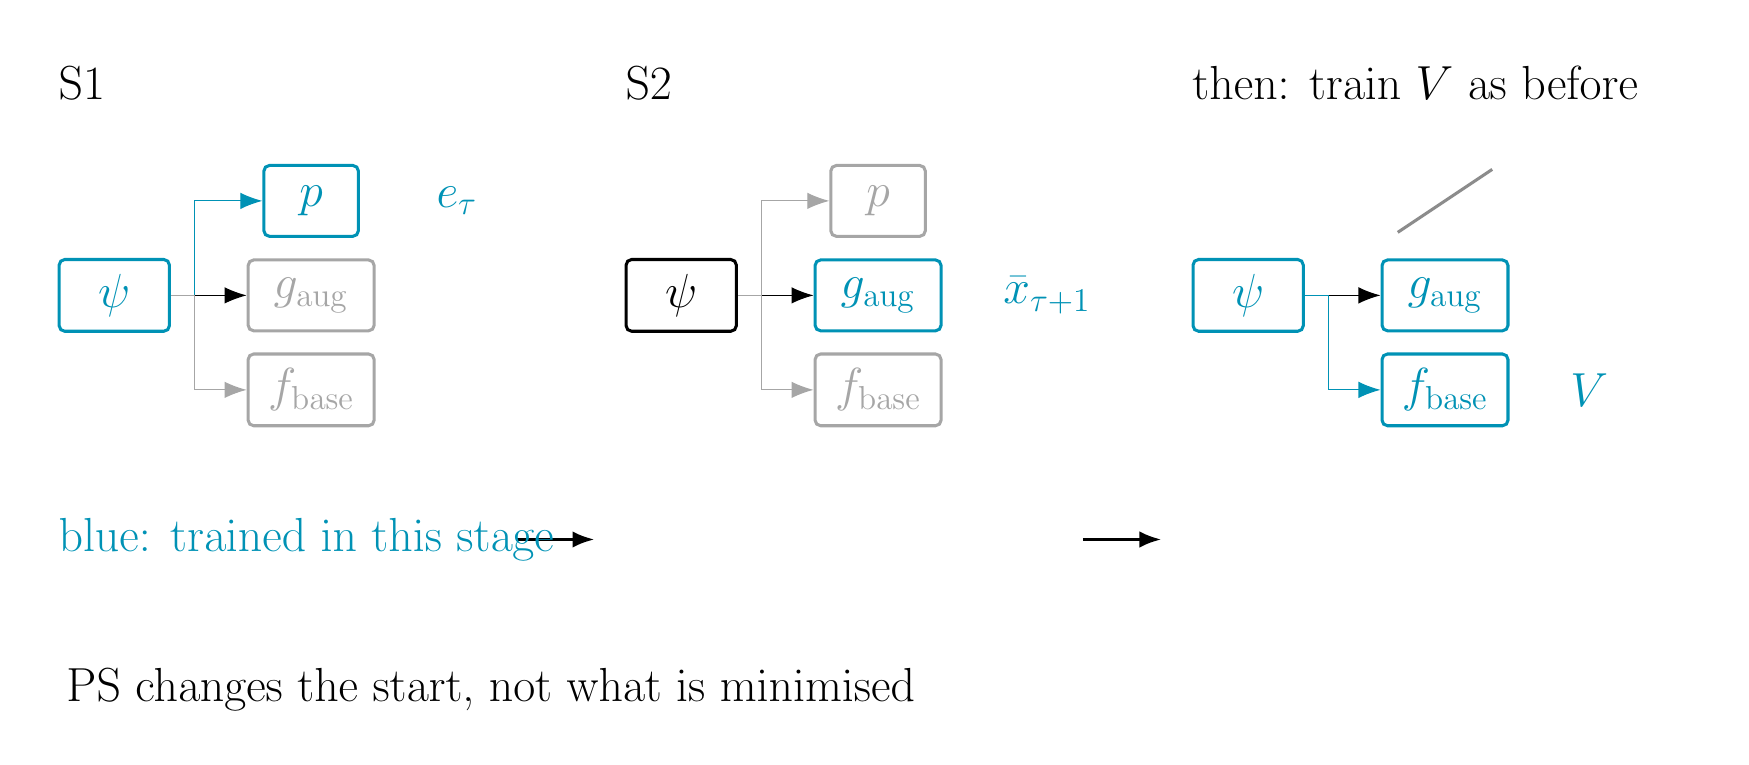
\begin{tikzpicture}
  \useasboundingbox (0,0) rectangle (21.5,9);
  \fontsize{17}{20}\selectfont
  \foreach \x/\t in {0.2/{S1}, 7.4/{S2}, 14.6/{then: train $V$ as before}}
    \node[anchor=west] at (\x,8.3) {\t};
  % panel glyph: psi -> xbar -> {p, g_aug}; colour per panel
  \newcommand{\panel}[5]{% x0, psi colour, p colour, g colour, f colour
    \node[blk, draw=#2, minimum width=1.4cm, minimum height=0.9cm] (a) at ({#1+0.9},5.6) {\color{#2}$\psi$};
    \node[blk, draw=#3, minimum width=1.2cm, minimum height=0.9cm] (b) at ({#1+3.4},6.8) {\color{#3}$p$};
    \node[blk, draw=#4, minimum width=1.6cm, minimum height=0.9cm] (c) at ({#1+3.4},5.6) {\color{#4}$g_{\mathrm{aug}}$};
    \node[blk, draw=#5, minimum width=1.6cm, minimum height=0.9cm] (d) at ({#1+3.4},4.4) {\color{#5}$f_{\mathrm{base}}$};
    \draw[->, #3] (a.east) -- ++(0.3,0) |- (b.west);
    \draw[->] (a.east) -- (c.west);
    \draw[->, #5] (a.east) -- ++(0.3,0) |- (d.west);}
  \panel{0.2}{hl}{hl}{black!35}{black!35}
  \node[anchor=west, text=hl] at (5.0,6.8) {$e_\tau$};
  \panel{7.4}{black}{black!35}{hl}{black!35}
  \node[anchor=west, text=hl] at (12.2,5.6) {$\bar x_{\tau+1}$};
  \panel{14.6}{hl}{white}{hl}{hl}
  \draw[black!45, line width=1.1pt] (17.4,6.4) -- (18.6,7.2);
  \node[anchor=west, text=hl] at (19.4,4.4) {$V$};
  \draw[->, line width=1.3pt] (6.2,2.5) -- (7.2,2.5);
  \draw[->, line width=1.3pt] (13.4,2.5) -- (14.4,2.5);
  \node[anchor=west, text=hl] at (0.2,2.5) {blue: trained in this stage};
  \node[anchor=west] at (0.3,0.6) {PS changes the start, not what is minimised};
\end{tikzpicture}
\end{document}
